\subsection{Constraint satisfaction problems}

\Blue{Factor graph} (aka Markov random field) a set of \underline{variables} $X
= {X_1,\dots,X_n}$ where $X_i \in \text{Domain}_i$ and \underline{factors}
$f_1,\dots,f_m$, with each $f_j(X) \ge 0$.
\Hint{Each factor is implemented as checking a solution rather than computing
the solution.}

\Green{Domain} possible values to be assigned to a variable.

\Red{Scope of a factor $f_j$} the set of variables $f_j$ depends on.
\Red{Arity} the size of this set. ``Unary factors'' (arity 1); ``Binary
factors'' (arity 2). ``Constraints'' (factors that return 0 or 1).

\Blue{Assignment weight} each \underline{assignment $x = (x_1, \dots, x_n)$}
yields a $\text{Weight}(x)$ defined as being the product of all factors $f_j$
applied to that assignment.
\fbox{$\text{Weight}(x) = \Pi_{j=q}^{m} f_j(x)$} ($x$ in its entirety is passed
in to each $f_j$ for simplicity of this notation, though in reality only a
subset of $x$ would be needed for $f_j$)

\Green{CSP} a factor graph where all factors are binary.
\fbox{For $j = 1,\dotsm$, $f_j(x) \in \{0,1\}$} (the constraint $j$ with
assignment $x$ is said to be satisfied iff $f_j(x) = 1$.)

\Green{Consistent assignment $x$ of a CSP} iff $\text{Weight}(x) = 1$ (i.e., all
constrains are satisfied.)

\Green{Dependent factors $D(x,X_i)$} a set of factors depending on $X_i$ but not
on unassigned variables.

\Red{Backtracking search} find maximum weight assignment of a factor graph.
\textbf{$\text{Backtrack}(x, w, \text{Domains})$}
\begin{enumerate}
    \item choose an unassigned \textbf{variable} $X_i$ \Hint{(MCV)}
    \item order \textbf{values} of $X_i$'s Domain \Hint{(LCV)}
    \item for each value $v$ in the order:\begin{enumerate}
        \item $\delta \leftarrow \Pi_{f_i\in D(x,X_i)}f_j(x\cup\left\{X_i:v\right\})$
        \item if $\delta = 0$: continue
        \item $\text{Domains}' \leftarrow \text{Domains}$ via \textbf{lookahead} \Hint{(forward checking)}
        \item if $\text{Domains}_i'$ is empty: continue
        \item \textbf{$\text{Backtrack}(x \cup \left\{X_i:v\right\}, w\delta, \text{Domains}')$}
    \end{enumerate}
\end{enumerate}
\begin{itemize}
    \item Strategy: extends partial assignments
    \item Optimality: exact
    \item Time: exponential
\end{itemize}

\Blue{Forward checking} one-step lookahead heuristic that preemptively removes
inconsistent values from the domains of neighboring variables.
\begin{itemize}
    \item After assigning a variable $X_i$, it eliminates inconsistent values from the domains of all its neighbors.
    \item If any of these domains become empty, stop the local backtracking search.
    \item if we unassign a variable $X_i$, have to restore the domain of its neighbors.
\end{itemize}

\Green{Most constrained \underline{variable}} selects the next unassigned
variable that has the fewest consistent values: fail early, prune early.
\Hint{Useful when some factors are constraints.}

\Green{Least constrained \underline{value}} assigns the next value that yields
the highest number of consistent values of neighboring variables: prefers the
value that is most likely to work. \Hint{Useful when all factors are
constraints.} If some factors get arbitrary non-negative values, we need to try
all consistent values anyway.

\Green{Arc consistency of variable $X_i$} w.r.t. $X_j$ is enforced when for each
$x_i \in \text{Domain}_i$, there exists $x_j \in \text{Domain}_j$ such that any
factos between $X_i$ and $X_j$ is non-zero.
\Hint{\textbf{Arc consistency is a \emph{definition}}, not an algorithm: enforce
all the way.}

\Red{AC-3} a multi-step lookahead heuristic that applies forward checking to all
relevant variables. After a given assignment, it performs forward checking and
then successively enforces arc consistency w.r.t. the neighbors of variables for
which the domain change during the process.
\Hint{AC-3 only looks locally at the graph for nothing blatantly wrong; it can't
detect when there are no consistent assignments.}

\Red{Beam search} extends partial assignments of $n$ variables of branching
factor $b = |\text{Domain}|$ by exploring the $K$ top paths at each step. The
beam size $1 \ge K \ge b^n$ controls the tradeoff between efficiency and
accuracy.
\Hint{Runtime is Linear to $n$: $O(n \underbrace{Kb
\log(Kb)}_{\text{sorting top K}})$}. $K=1$: greedy search ($O(nb)$ time); $K
\rightarrow +\infty$: BFS ($O(b^n)$ time).
\begin{itemize}
    \item Strategy: extends partial assignments
    \item Optimality: approximate
        \Hint{
            \begin{itemize}
                \item Global optimality is only guaranteed by unbounded beam size
                \item Increasing $k$ from 1 to 2 doesn't guarantee increasing weight assignment
            \end{itemize}
        }
    \item Time: linear
\end{itemize}

\Blue{Local search (iterated conditional modes)} modifies the assignment of a
factor graph one variable at a time until convergence. At step $i$, assign to
$X_i$ the value $v$ that maximizes the product of all factors connected to that
variable.
\begin{itemize}
    \item Initiualize $x$ to a random complete assignment (not partial)
    \item Loop through $i = 1, \dots, n$ until convergence: \begin{itemize}
        \item Compute weight of $x_v = x \cup {X_i :v}$ for each $v$
        \item $x \leftarrow x_v$ with highest weight
    \end{itemize}
\end{itemize}
\Hint{ICM may get stuck in local optima; adding randomness may help.}
\begin{itemize}
    \item Strategy: modify complete assignments
    \item Optimality: approximate
    \item Time: linear
\end{itemize}

\Red{CSP tricks}
\Hint{
    \begin{itemize}
        \item If it's possible that a variable doesn't get an assignment,
            consider extending the domain to inclue a $\emptyset$ value.
        \item max weight assignment may be skewed towards arbitrarily high
            assignment if there exists unbounded non-negative factor value like
            a ``preference''. Bounding it to say 1 through 10 may help.
    \end{itemize}
}

\subsection{Markov Networks}

\begin{tabular}{|c|c|c|c|} 
    \hline
    \textbf{CSPs} & \textbf{Markov networks} \\
    \hline
    variables & random variables \\ 
    \hline
    weights & probabilities \\
    \hline
    max weight assignment & marginal probabilities \\
    \hline
\end{tabular}

Capture the uncertainty over assignment using the language of probability.

\Green{Markov Network} a factor graph which defines a joint distribution over
random variables $X = (X_1,\dots,X_n)$:
\fbox{$\mathbb{P}(X=x)=\frac{\text{Weight}(x)}{Z}$}

\Green{$Z = \sum_{x'} \text{Weight}(x')$} sum all the possible assignments'
weights (normalization constant)

\Green{Marginal probability} the probability of when one particular variable
$X_i$ is assigned with a particular value $v$: sum $\mathbb{P}$ when $X_i = v$
\fbox{$\mathbb{P}(X_i=v)=\sum_{x:x_i=v}\mathbb{P}(X=x)$}

\Blue{Gibbs sampling} approximately computes marginal probabilities.
\Hint{Follows the tempalte of local search: change one variable at a time. But
unlike ICM, Gibbs is a randomized algo .}

\begin{itemize}
    \item Initialize $x$ to a random complete assignment.
    \item Loop through $i=1,\dots,n$ until convergence: \begin{itemize}
        \item Set $x_i = v$ with probability $\mathbb{P}(X_i = v | \underbrace{X_{-i}}_{\text{all vars except} X_i}=x_{-i})$
        \item Increment $\text{count}_i(x_i)$ (how often this assignment is encountered. \Hint{can just track particular vars we're interested in.})
    \end{itemize}
    \item Estimate $\hat{\mathbb{P}}(X_i=x_i)=\frac{\text{count}_i(x_i)}{\sum_{v}\text{count}_i(v)}$
\end{itemize}

\begin{tabular}{|c|c|}
    \hline
    \textbf{ICM} & \textbf{Gibbs sampling} \\
    \hline
    max weight & marginal probabilities \\ 
    assignment &   \\ 
    \hline
    choose best value & sample a value \\
    \hline
    converges to & marginals converge to\\
    local optimum & correct answer \\
    \hline
\end{tabular}

\subsection{Bayesian Networks}

\boxed{
    P(A|B,C) = \frac{P(B|A,C) P(A|C)}{P(B|C)}
}

\Blue{Explaining away} suppose two causes positively influence an effect.
Conditioned on the effect, further conditioning on one causes reduces the
probability of the other cause.

\Red{Bayesian network} a directed acyclic graph that specifies a joint distribution
over random variables $X=(X_1,\dots,X_n)$ as a product of local conditional distributions,
one for each node: \fbox{$\mathbb{{P}}(X_1=x_1,\dots,X_n=x_n) = \prod_{i=1}^{n}
p(x_i|x_{\text{Parents}(i)})$}

\Blue{Probabilistic program} randomizes variable assignment such that we can
write down complex Bayesian networks that generates assignments without having
to explicitly specify associated probabilities.
\Hint{Unlike normal classification (e.g., neural nets), Bayesian networks
provide a different paradigm where we think about going from output to the
input.}

\Green{Probabilistic inference strategy} to compute the probability $P(Q|E=e)$
of query $Q$ given evidence $E=e$:
\begin{enumerate}
    \item Remove vars that aren't ancestors of the query $Q$ or the evidence $E$ by marginalization
    \item Convert Bayesian network to factor graph
    \item Condition on the evidence $E=e$
    \item Remove nodes disconnected from the query $Q$ by marginalization
    \item Run probabilistic inference algorithm
\end{enumerate}
\Blue{Filtering question} asks for the distribution of some hidden variable
$H_i$ conditioned on only the evidence up until that point. \Hint{Useful for
real-time object tracking as the future can't be seen.}
\Blue{Smoothing question} asks for the distribution of some hidden variable
$H_i$ conditioned on on the evidence including the future. \Hint{Useful when all
the data have been collected and we want to retrospectively go and figure out
what the hidden state $H_i$ was.}

\Green{Lattice representation} $O(n|\text{Domain}|)$ nodes and
$O(n|\text{Domain}|^2)$ edges.
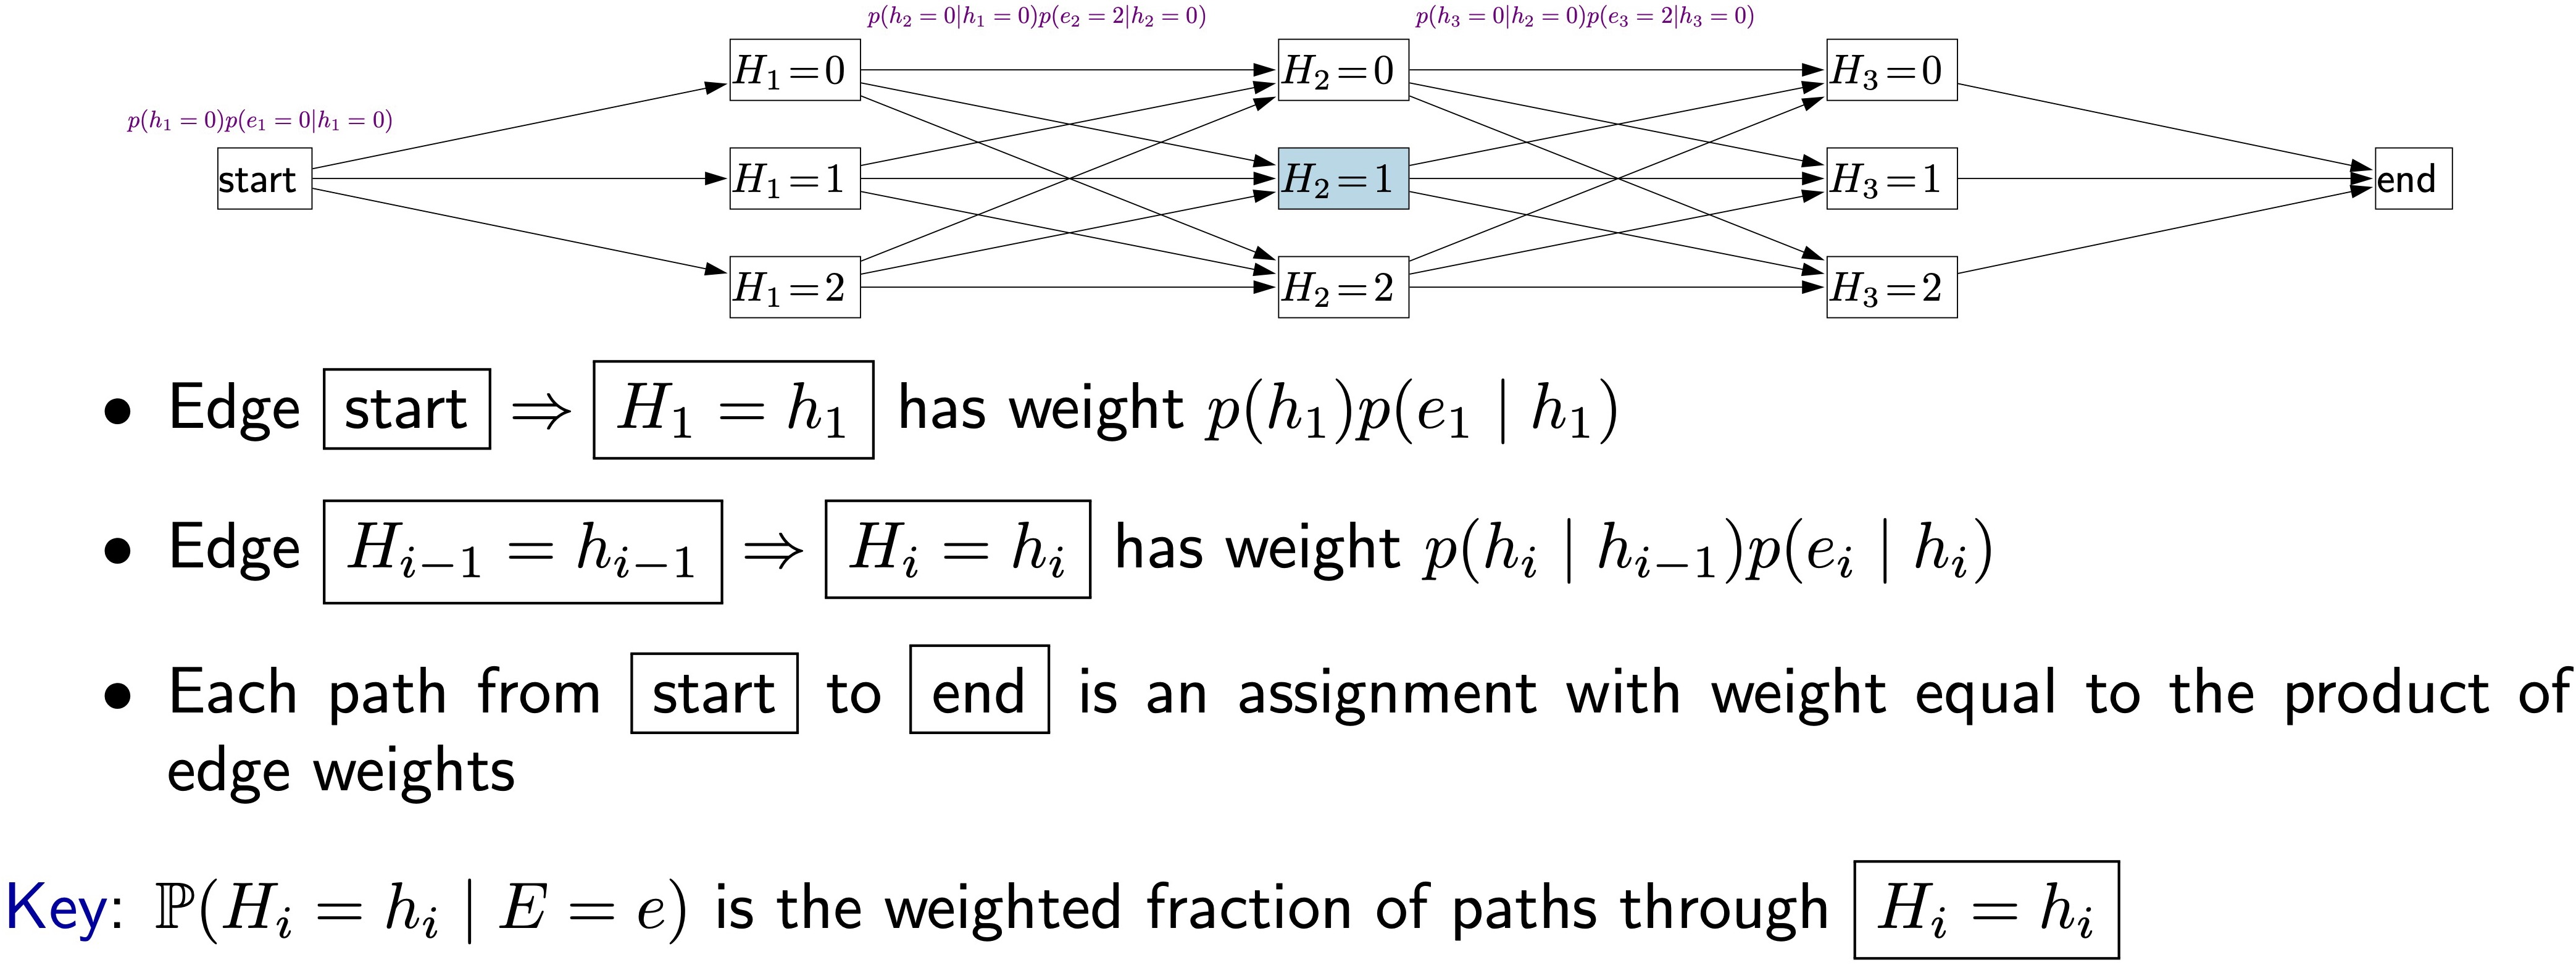
\includegraphics[width=0.25\textwidth]{topics/lattice_representation.jpg}
A path's weight is also the joint probability $P(H=h,E=e)$ (all variables assigned!)

\Red{Forward-backward algorithm} computes the exact value of $P(H=h_k|E=e)$ a
smoothing query) for any $k\in\left\{1,\dots,L\right\}$ in the case of an HHM of
size $L$. \Hint{Running time: $O(n|\text{Domain}|^2)$.}
\begin{enumerate}
    \item for $i\in \left\{1,\dots,L\right\}$, compute $F_i(h_i)=$\\
        \fbox{
            $\begin{cases}
            p(h_1)p(e_1|h_1) & i = 1\\
            \sum_{h_{i-1}}F_{i-1}(h_{i-1})p(h_i|h_{i-1})p(e_i|h_i) & \text{otherwise}\\
            \end{cases}$
        }
    \item for $i\in \left\{L,\dots,1\right\}$, compute $B_i(h_i)=$\\
        \fbox{
            $\begin{cases}
                1 & $i = n$\\
                \sum_{h_{i+1}}B_{i+1}(h_{i+1})p(h_{i+1}|h_i)p(e_{i+1}|h_{i+1}) & \text{otherwise}\\
            \end{cases}$
        }
    \item for $i\in \left\{1,\dots,L\right\}$, compute $S_i(h_i)=\frac{F_i(h_i)B_i(h_i)}{\sum_{h_i}F_i(h_i)B_i(h_i)}$
\end{enumerate}
with the convention $F_0 = B_{L+1}$. We get \fbox{$P(H=h_k|E=e) = S_k(h_k)$}

\Green{Particle (partial assignment) filtering} approximates the posterior
density of state variables given the evidence of observation variables by
keeping track of $K$ particles at a time. Initialize $C \leftarrow
\left[\left\{\right\}\right]$. For $t = 1,\dots,n$:
\begin{enumerate}
    \item \textbf{proposal:} for each old particle $x_{t-1} \in C$, sample $x$
        from the transition probability distribution $p(x|x_{t-1})$ and add $x$
        to a set $C'$.
    \item \textbf{weighting:} weight each $x$ of the set $C'$ by $w(x) =
        p(e_t|x)$ ($e_t$ is the evidence observed at time $t$).
    \item \textbf{resampling:} sample $K$ elements from the set $C'$ using the
        probability distribution induced by $w$ and store them in $C$: these are
        current particles $x_t$.
\end{enumerate}

\Green{Maximum likelihood} if we don't know the local conditional distributions,
we can learn them using max likelihood.
\fbox{$\max_\theta \prod_{x \in D_{\text{train}}} p(X = x;\theta)$}
\Hint{HMM parameters: $\theta = (p_{\text{start}}, p_{\text{trans}},
p_{\text{emit}})$.}

\Green{Laplace smoothing} for each distribution $d$ and partial assignment 
$(x_{\text{Parents}(i)}, x_i)$, add $\lambda$ (a constant) to
$\text{count}_{d}(x_{\text{Parents}(i)}, x_i)$, then normalize to get
probability estimates.
\Hint{Hallucinate $\lambda$ occurrences of each local assignment.}
Larger $\lambda$ $\Rightarrow$ more smoothing $\Rightarrow$ probabilities closer
to uniform.

\Red{Expectation-Maximization (EM)} a parameter \Hint{learning algorithm} that
estimates the parameter $\theta$; $H$ is hidden, $E=e$ is observed:
\begin{itemize}
    \item Initialize $\theta$ randomly
    \item Repeat until convergence:\begin{itemize}
        \item \underline{E-step}:\begin{itemize}
            \item Compute \fbox{$q(h) = P(H=h|E=e;\theta)$}
            \item Create fully-observed weighted examples: $(h, e)$ with weight
                $q(h)$
        \end{itemize}
        \item \underline{M-step}: Maximum likelihood (count and normalize) on
            weighted examples to get $\theta$
    \end{itemize}
\end{itemize}
One iteration of EM:
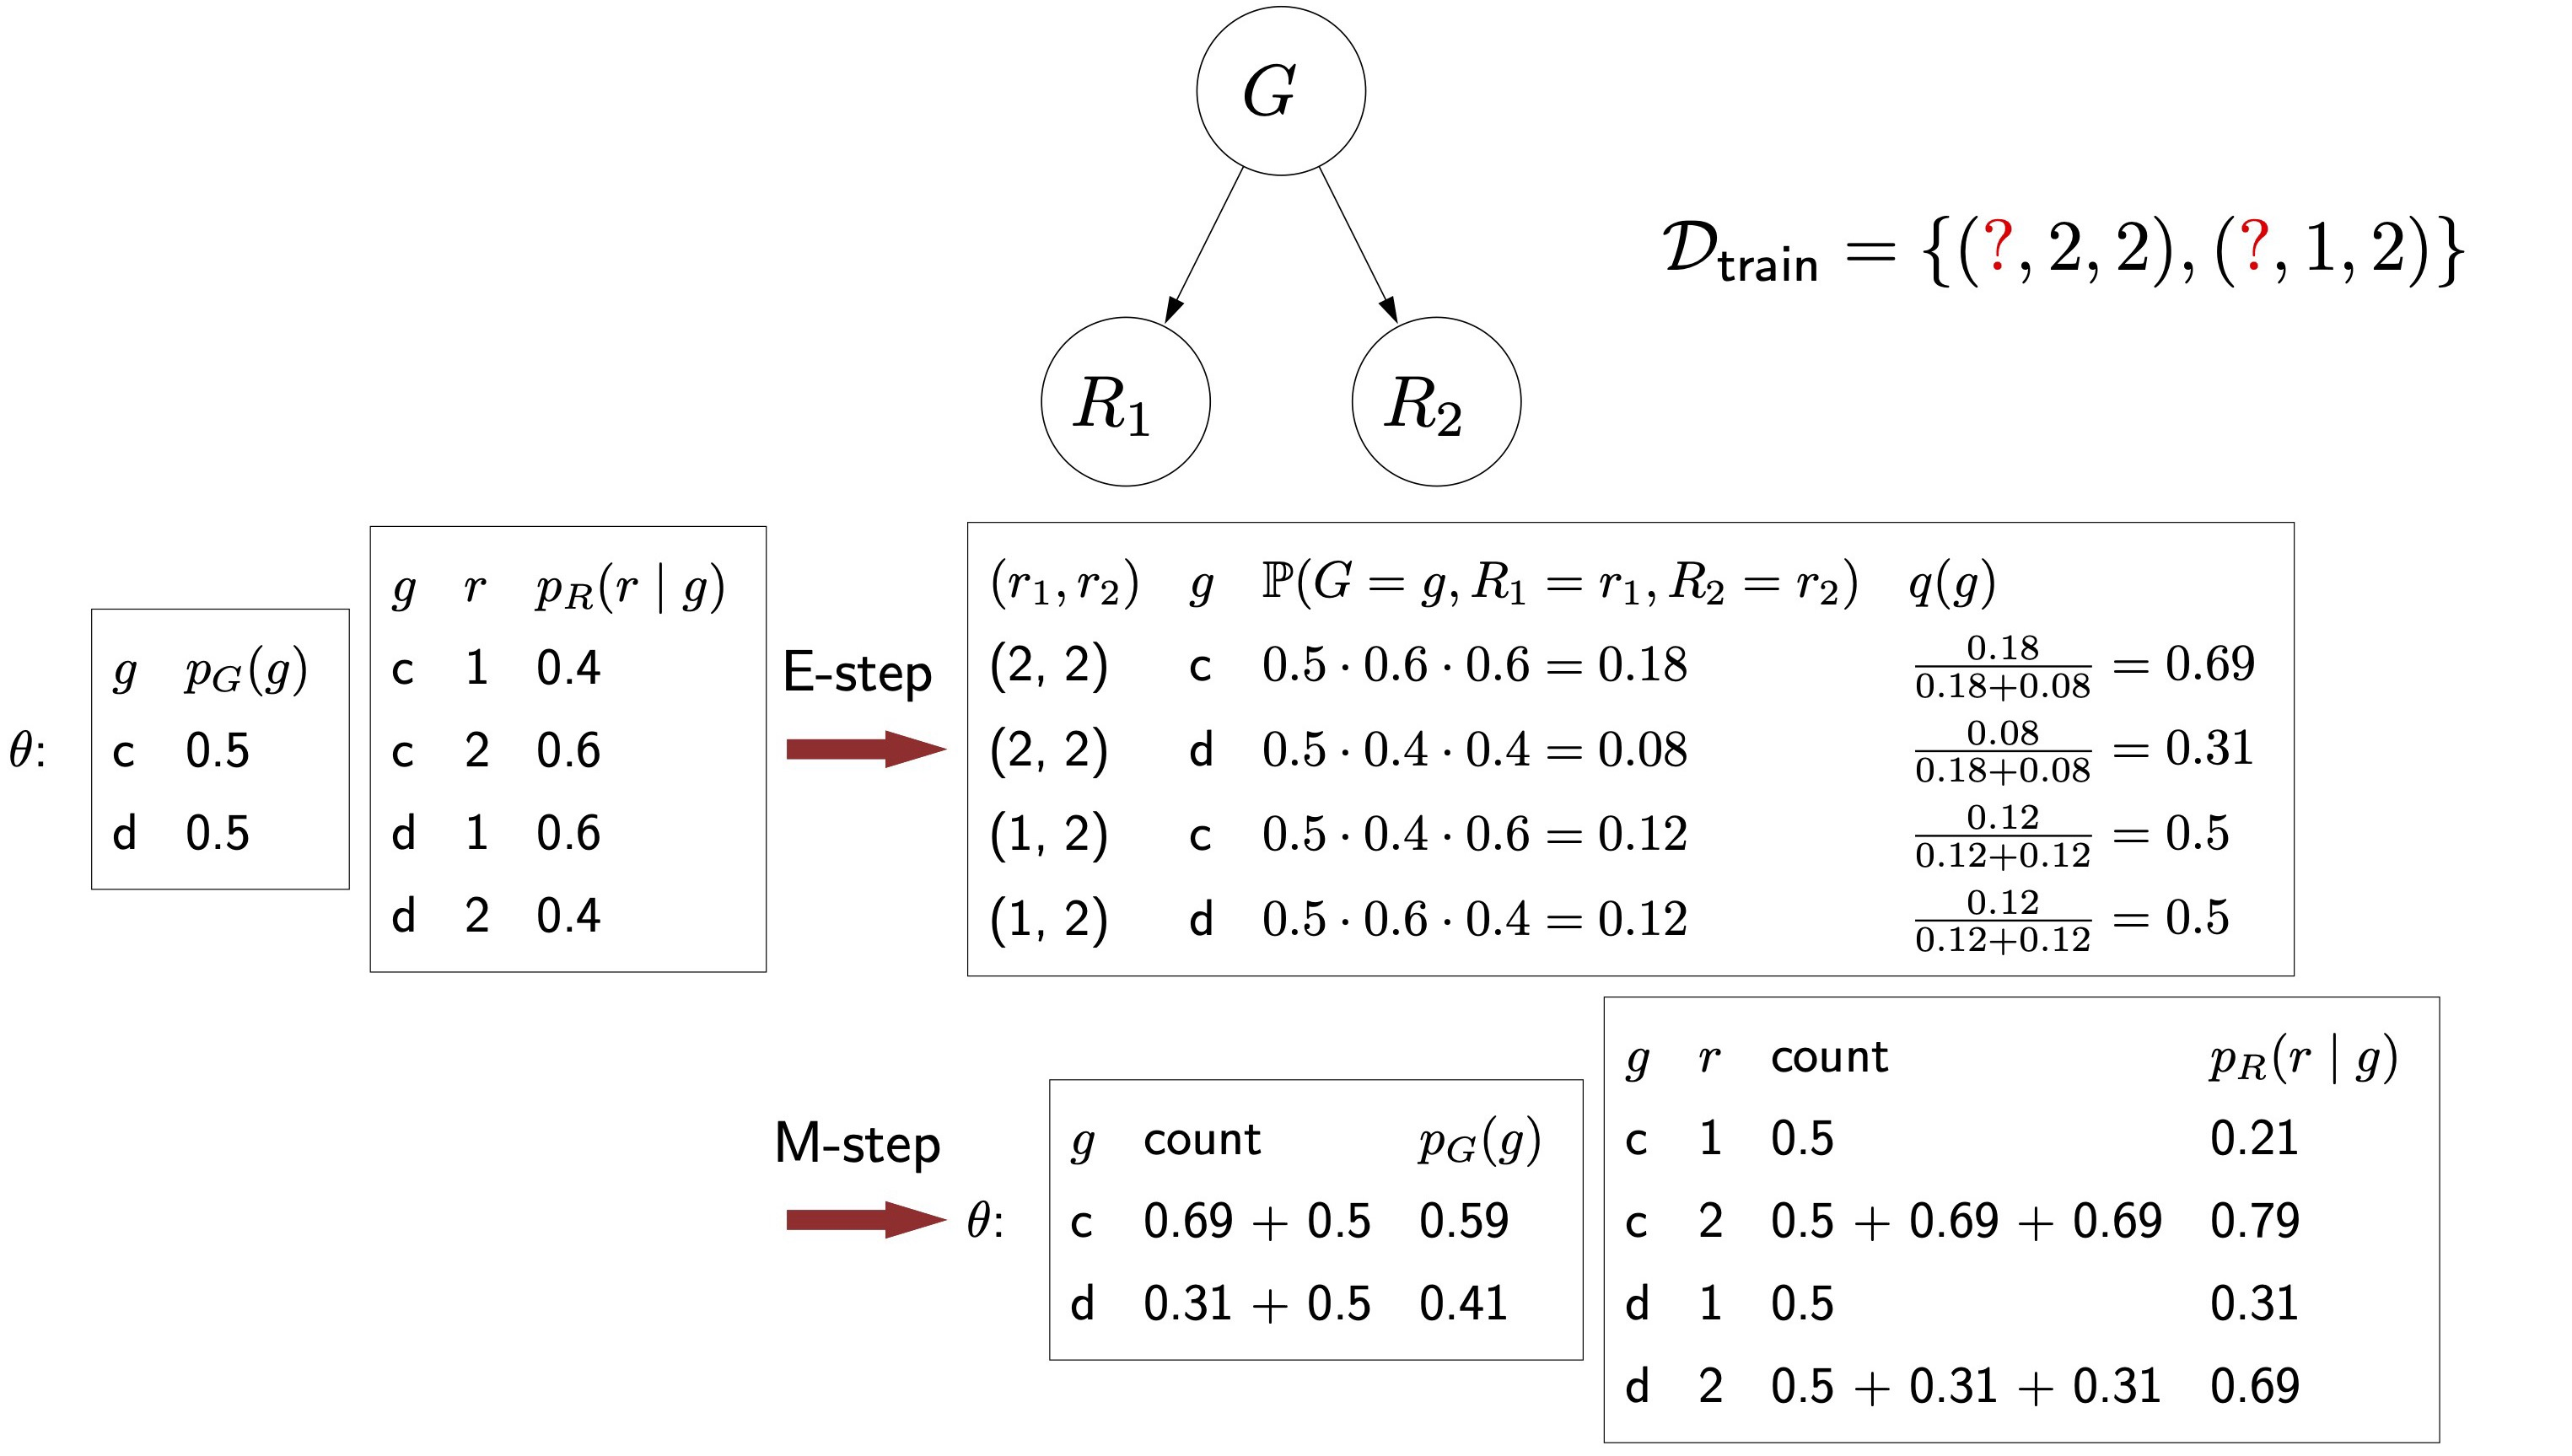
\includegraphics[width=0.25\textwidth]{topics/em.jpg}
\Hint{Like K-means, EM converges to a local optima. \textbf{EM can handle partial data.}}

\begin{wrapfigure}{l}{0.12\textwidth}
    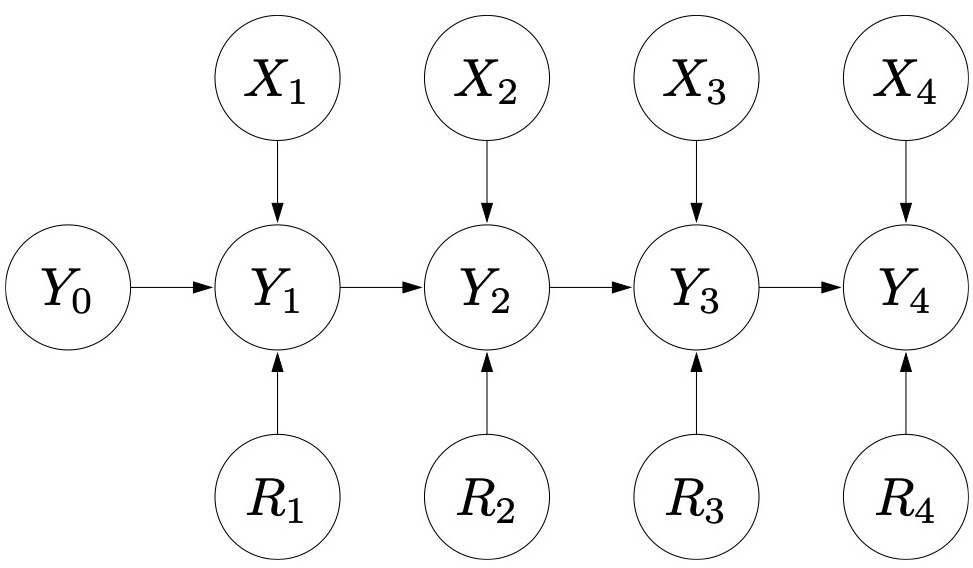
\includegraphics[width=0.12\textwidth]{topics/Bayesnet_problem.jpg}
\end{wrapfigure}
$Y_0 = 0$\\
$X_i$ chosen uniformly from $\{1,2,3,4\}$. \\
$p(R_i = 1) = (1-\epsilon)$ (remember)\\
\textbf{Suppose we observe that $Y_2=3$. What do we believe about $X_2$?}\\
First note that $Y_1=X_1$ deterministically, which has a uniform distribution
over $\{1, 2, 3, 4\}$. Next, let us write out the conditional distribution:
$P(X_2=x_2|Y_2=3) \propto P(X_2=x_2, Y_2=3) = \sum_{y_1,r_2} p(y_1)p(r_2)p(x_2)p(y_2=3|y_1,x_2,r_2)$
Now comute RHS for each value of $x_2$

\begin{wrapfigure}{l}{0.15\textwidth}
    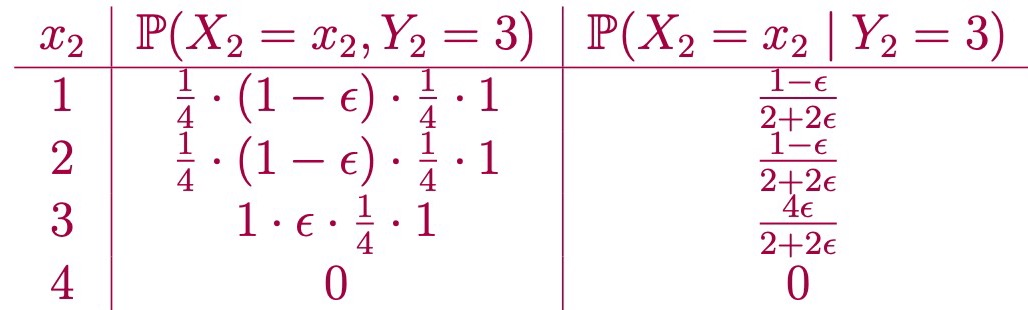
\includegraphics[width=0.15\textwidth]{topics/Bayesnet_problem_ans.jpg}
\end{wrapfigure}
For $X_2 \in \{1,2\}$, we must have had remembered ($R_2 = 1$), which forces
$Y_1 = Y_2 - X_2$ (has probability $\frac{1}{4}$). For $X_2=3$, we must have
forgotten ($R_2 = 0$), and $Y_1$ is free to be anything (has probability $1$).
